\begin{center}
Игра
\end{center}
Таблица <<games>>
\begin{tabular}{l@{\hspace{5mm}}l@{\hspace{5mm}}l@{\hspace{5mm}}l} \toprule
  Наименование & Тип  & Описание\\ 
\midrule
  id & int & Уникальный идентификатор\\
  uuid & varchar(255) & Глобальный Уникальный идентификатор\\
  title & varchar(255) & Заголовок\\
  type\_game & varchar(255) & Тип игры\\
  date\_create & datetime & Дата создания\\
  date\_start & datetime & Дата начала\\  
  date\_stop & datetime & Дата завершения\\
  date\_change & datetime & Дата изменения\\
  owner & varchar(255) & \\
  date\_restart & datetime & Дата перезапуска\\
  description & varchar(255) & Описание игры\\
  organizators & varchar(255) & Организаторы\\
  state & varchar(255) & Состояние\\
  form & varchar(255) & Форма проведения\\
  rules & varchar(255) & Правила игры\\
  maxscore & int & Максимальный счет\\
\bottomrule
\end{tabular}
\vspace{\baselineskip}


\begin{center}
Концепция игры Exploitation Quest
\end{center}

Ключевая идея данного типа игр заключается в моделировании работы информационных инфраструктур абстрактных организации. Общая сеть поделена на две обособленные логические части, непосредственно взаимодействующие между собой. В первой подсети располагаются запущенные сервисы, а во второй - боты, имитирующие деятельность персонала предполагаемой организации, совершающие отправку некоторых данных на сервисы и получающие от них ответы.\par
Подсистема оркестрации системы FreeHackQuest будет запускать ботов и развертывать сервисы в изолированном окружении с помощью диспетчера контейнеров LXD.\par
После завершения подготовительного этапа, участники соревнований допускаются до сети, где им предлагается попытаться выполнить различные задания (например повысить свои привилегии, получить доступ к сервисам или информации или контроль над всей сетью). Каждый раз, когда игрок справляется с поставленной перед ним задачей, ему начисляются очки рейтинга, которые определяют его место в общем зачете. По окончанию проведения соревнований участник с наибольшим рейтингом побеждает.\par
Также заработанные очки можно обменивать на подсказки в том случае, если в ходе выполнения заданий у игрока возникают трудности.\par
Условная схема концепции игры Exploitation Quest:

\begin{center}
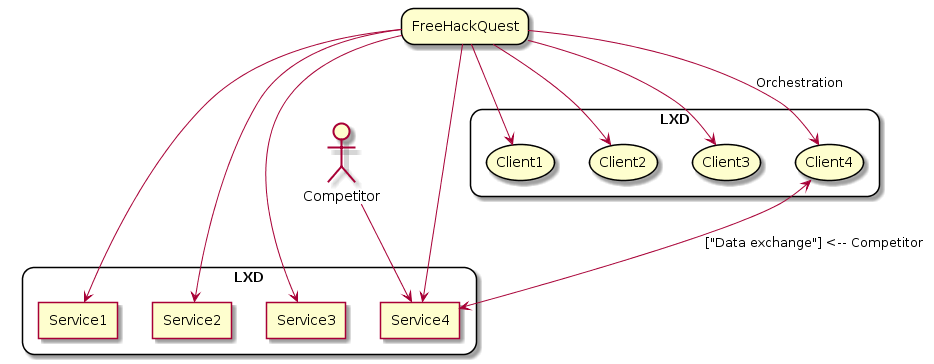
\includegraphics[width=0.65\textwidth]{eq}\\
Рисунок -- Exploitation Quest\\
\end{center}
\vspace{\baselineskip}

Система оркестрации является необходимым этапом для работы Exploitation quests - заданий на эксплуатацию. Она позволит развертывать сервисы с уязвимостями и запускать ботов, имитирующих поведение пользователей.\par
Система оркестрации позволяет отправлять HTTP GET, POST, PUT, DELETE запросы серверу LXD, а также создавать, получать, запускать, останавливать и удалять контейнеры, узнавать информацию о контейнере.\par

Система оркестрации является частью подсистемы сервера FreeHackQuest и имеет следующую структуру взаимодействия:
\begin{center}
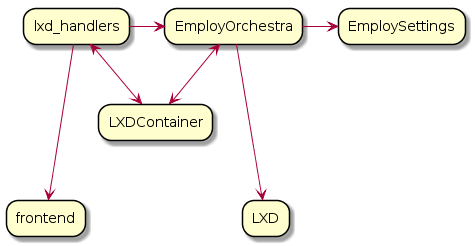
\includegraphics[width=0.65\textwidth]{orc}\\
Рисунок -- Структура взаимодействия системы оркестрации \\
\end{center}
\vspace{\baselineskip}

Диаграмма классов, используемых для системы оркестрации, в упрощенном виде:
\begin{center}
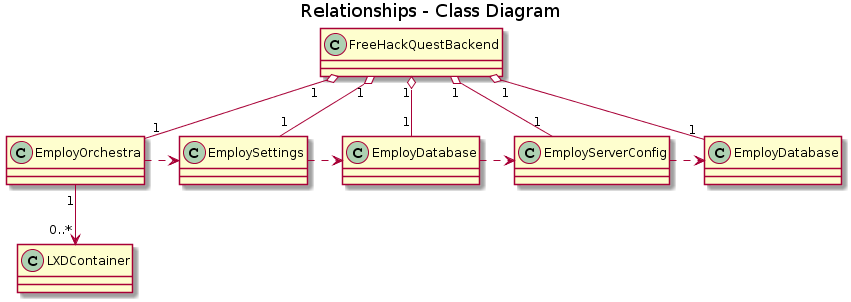
\includegraphics[width=0.65\textwidth]{orc_klass}\\
Рисунок -- UML диаграмма классов системы оркестрации \\
\end{center}
\vspace{\baselineskip}

Диаграмма класса EmployOrchestra:
\begin{center}
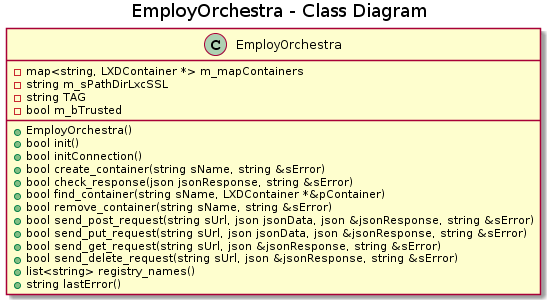
\includegraphics[width=0.65\textwidth]{eo_klass}\\
Рисунок -- Диаграмма класса EmployOrchestra \\
\end{center}
\vspace{\baselineskip}

Диаграмма класса LXDContainer:
\begin{center}
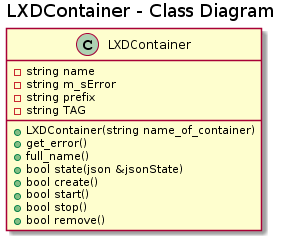
\includegraphics[width=0.65\textwidth]{lxdc_klass}\\
Рисунок -- Диаграмма класса LXDContainer \\
\end{center}
\vspace{\baselineskip}

Система виртуализации необходима для изолированного выполнения сервисов с уязвимостями, так как участники могут скомпрометировать машину, на которой развернута моделируемая инфраструктура организации. Система виртуализации должна обладать сетевым управлением, такое требование позволяет размещать контейнеры на отдельной от backend сервера машине.\par

\begin{center}
Система подсказок
\end{center}
Участвуя в соревнованиях по информационной безопасности, игроки зачастую тратят на отдельные задания чрезмерно много времени. Обычно это обусловлено усложненной логикой, заложенной разработчиком задачи, или же пробелами в теоретических знаниях (или практических умениях) у самого участника соревнований.\par
Для экономии времени игрокам, оказавшимся в подобных ситуациях, была разработана система “платных” подсказок к заданиям из игр. Приобретение подсказок осуществляется за очки рейтинга (при покупке очки отнимаются от общего счета игрока), заработанные участником в ходе соревнований. Система получила название Leaks (утечки).\par
Для реализации системы были разработаны три таблицы реляционной базы данных SQL.\par


Таблица <<leaks>>\par

\begin{tabular}{l@{\hspace{5mm}}l@{\hspace{5mm}}l@{\hspace{5mm}}l} \toprule
  Наименование & Тип  & Описание\\ 
\midrule
  id & int & Уникальный идентификатор\\
  uuid & varchar(255) & Глобальный Уникальный идентификатор\\
  gameid & int & Ссылка на игру\\
  name & varchar(255) & Видимая информация до покупки\\
  content & text(4096) & Описание “утечки” доступно только после того, как игрок “купит”\\
  score & int & За сколько очков можно “Купить”\\
  created & datetime & Дата создания\\
  updated & datetime & Дата последнего обновления\\
  sold & int & Сколько всего уже продано\\
\bottomrule
\end{tabular}

\vspace{\baselineskip}

Таблица <<users\_leaks>>\par

\begin{tabular}{l@{\hspace{5mm}}l@{\hspace{5mm}}l@{\hspace{5mm}}l} 
\toprule
  Наименование & Тип  & Описание\\
\midrule
  id & int & Уникальный идентификатор\\
  leakid & int & Ссылка на “утечку”\\
  userid & int & Ссылка на “Пользователя”\\
  grade & int & Оценка “утечки” пользователем\\
  dt & datetime & Точное время приобретения\\
\bottomrule
\end{tabular}

\vspace{\baselineskip}

Таблица <<leaks\_files>>\par

\begin{tabular}{l@{\hspace{5mm}}l@{\hspace{5mm}}l@{\hspace{5mm}}l} 
\toprule
Наименование & Тип  & Описание\\
\midrule
  id & int & Уникальный идентификатор\\
  uuid & varchar(255) & Глобальный Уникальный идентификатор\\
  leakid & int & Ссылка на “утечку”\\
  filename\_orig & varchar(255) & Оригинальное имя файла\\
  md5 & varchar(255) & MD5 сумма от файла\\
  size & int & Размер файла\\
  dt & datetime & Дата\\
  filepath & varchar(255) & Путь до файла “утечки”\\
\bottomrule
\end{tabular}

\vspace{\baselineskip}

\begin{center}
Пользователь
\end{center}

\begin{tabular}{l@{\hspace{5mm}}l@{\hspace{5mm}}l@{\hspace{5mm}}l} 
\toprule
Наименование & Тип  & Описание\\
\midrule
  id & int & Уникальный идентификатор\\
  uuid & varchar(255) & Глобальный Уникальный идентификатор\\
  email & varchar(255) & E-mail пользователя\\
  password & varchar(255) & Пароль пользователя\\
  role & varchar(255) & Роль\\
  nick & varchar(255) & Имя пользователя\\
  logo & varchar(255) & \\
  dt\_create & datetime & Дата создания\\
  dt\_last\_login & datetime & Дата последнего входа\\
  last\_ip & varchar(255) & IP пользователя\\
  status & varchar(255) & Статус\\
  country & varchar(255) & Страна\\
  region & varchar(255) & Регион\\
  city & varchar(255) & Город\\
  latitude &  & \\
  longtitude &  & \\
  rating & int & Рейтинг пользователя\\
  about & string & Дополнительная информация о пользователе\\
  university & varchar(255) & Университет\\
\bottomrule
\end{tabular}
\vspace{\baselineskip}

Модель данных и взаимодействия выглядит следующим образом:
\begin{center}

Рисунок --  \\
\end{center}
\vspace{\baselineskip}

\begin{center}
Задача
\end{center}

\begin{tabular}{l@{\hspace{5mm}}l@{\hspace{5mm}}l@{\hspace{5mm}}l} 
\toprule
Наименование & Тип  & Описание\\
\midrule
  idquest & int & Уникальный идентификатор\\
  uuid & varchar(255) & Глобальный Уникальный идентификатор\\
  name & varchar(255) & Название задачи\\
  text & varchar(255) & Формулировка задачи\\
  answer & varchar(255) & Ответ\\
  score & int & Счет\\
  author & varchar(255) & Автор\\
  subject & varchar(255) & \\
  answer\_upper\_md5 & varchar(255) & Ответ в зашифрованном виде\\
  gameid & int & Уникальный идентификатор игры\\
  state & varchar(255) & Состояние\\
  description\_state & varchar(255) & Описание состояние\\
  city & varchar(255) & Город\\
  date\_change & datetime & Дата изменения\\
  date\_create & datetime & Дата создания\\
  userid & int & Уникальный идентификатор пользователя\\
  count\_user\_solved & int & Количество пользователей, решивших задачу\\
  copyright & varchar(255) & Авторство\\
  answer\_format & varchar(255) & Формат ответа\\
\bottomrule
\end{tabular}
\vspace{\baselineskip}

\begin{center}
Сдача задания
\end{center}

\begin{center}
Обновление задания
\end{center}
Алгоритм расчета рейтинга пользователя

\begin{center}
Удаление задания
\end{center}

